%! suppress = FileNotFound
\documentclass[../main]{subfiles}

\begin{document}

\chapter{A testing framework for Scratch}\label{ch:itch}

\dictum[Larry Flon \\ \textit{On research in structured programming}]{There does not now, nor will there ever, exist a programming language in which it is the least bit hard to write bad programs.}

Block-based languages like Scratch are popular tools for introducing computer science concepts to young learners~\autocite{bauLearnableProgrammingBlocks2017,zhangSystematicReviewLearning2019}.
The intuitive interface and focus on visuals make Scratch an engaging and accessible programming environment.
Due to this visual nature, syntactical programming errors are eliminated and students can quickly create games, stories, or other projects.
This approach gives students a lot of flexibility to express their creativity.
However, functional errors will still occur~\autocite{zellerWhyProgramsFail2009a}.
The process of teaching to code is often slowed down by the delay in providing feedback on and solutions to these errors.

When done manually, assessment of submissions for Scratch exercises is time-consuming and impractical, especially in large classes, where educators often lack the time to give individual feedback to each student.
That is why it is important to equip students with tools that can provide immediate feedback and thus enhance their independent learning skills.
In this chapter, we introduce Itch, a testing framework for Scratch that can act as an automated assessment tool~\autocite{douceAutomaticTestbasedAssessment2005}.

Itch provides flexible testing capabilities: it supports both static and dynamic testing of Scratch projects.
It also provides facilities to make common scenarios easy to test, allowing the educators to focus on testing the interesting parts of an exercise.
We also reflect on Itch's use in an educational context and discuss what testing of Scratch exercises should look like.
On the one hand, Scratch strives to allow maximal creative expression for students, while on the other hand, testable exercises need a well-defined goal and reasonable limits.

\section{Related work}\label{sec:related-work}

In this section, we look at the few existing testing frameworks for Scratch.
Since they are few and far between, we also consider other tools with similar aims: helping students with Scratch.
We begin by looking at the linter-like tools that perform static analysis.

One of the first ones is Hairball~\autocite{boeHairballLintinspiredStatic2013}.
Hairball analyses the blocks of a provided Scratch project, with multiple rules and analyzers available.
Dr.\ Scratch~\autocite{moreno-leonDrScratchWeb2015} allows analysing a Scratch project to provide various insights.
For example, Dr.\ Scratch uses Hairball to assign a ``computational thinking score'' to the project, although the creators of Scratch are not a fan of this approach~\autocite{resnickCodingCrossroads2020}, see \cref{subsec:how-to-evaluate-scratch-submissions}.

QualityHound~\autocite{techapalokulQualityHoundOnline2017} is a linter that detects code smells like ``duplicate code'' or ``broad variable scope''.
In total, twelve code smells are detected.
LitterBox~\autocite{fraserLitterBoxLinterScratch2021} is a newer linter that shares some goals with QualityHound.
For example, it will also detect code smells.
LitterBox supports significantly more patterns, and also finds potential bugs~\autocite{fradrichCommonBugsScratch2020}, by looking for code that seems suspicious (for example, comparing two literal values).
Subsequent research has expanded LitterBox to find ``code perfumes''~\autocite{obermullerCodePerfumesReporting2021}, which provides positive feedback to students, for example, by noting good use of loops.

LitterBox can also translate code to LeILa, an intermediate language of the Bastet framework~\autocite{stahlbauerVerifiedScratchProgram2020}.
Bastet uses this intermediate language to enable more traditional and advanced analysis and verification of Scratch programs.
Examples of what the authors envision are automated test generation, data-flow analysis, unbounded model checking on predicate abstraction, and concolic testing.

\marginnote{Unfortunaly, we were not aware of \textsc{itch} when deciding to name our testing framework Itch.}
\textsc{itch}~\autocite{johnsonITCHIndividualTesting2016} is the first automatic testing framework to the knowledge of the authors.
It translates a very limited subset of Scratch programs to Python.
\textsc{itch} uses the Scratch say and ask functionality to perform input/output-based testing on Scratch projects.
Of course, being limited to input/output, only a subset of the functionality of Scratch can be used.

Finally, Whisker~\autocite{stahlbauerTestingScratchPrograms2019} is a fully automated testing framework for Scratch, and the most similar to Itch.
While manually written test suites (also in JavaScript) are possible, Whisker focuses on automated testing~\autocite{deinerAutomatedTestGeneration2023}.
For example, Whisker (and subsequent research), supports property-based testing, search-based testing~\autocite{deinerSearchBasedTestingScratch2020}, and model-based testing~\autocite{gotzModelbasedTestingScratch2022}.

\section{Introduction to Itch}\label{sec:introduction-to-itch}

Itch is an educational testing framework for Scratch exercises.
Educators can write test suites (in JavaScript) that evaluate a submission to determine if the submission correctly implements the requirements in the problem statement of the exercise.
A submission is the code (in this case the Scratch project) that students submit as the answer to a programming exercise.

Broadly, Itch provides two approaches to testing, static and dynamic tests.
For the static tests, the project is not run: only the blocks are considered.
With static tests, the test suite can verify (discussed in \cref{subsec:before-execution}):

\begin{itemize}[noitemsep]
    \item If the students did not change some off-limit sprites.
    \item The metadata of the sprites, which sprites exist, their position, their size, their costume, et cetera.
    \item All kinds of checks on the blocks: only certain blocks were used, some blocks were not used, the blocks must match a particular pattern, the number of blocks, and so on.
\end{itemize}

However, the most flexible option is to use dynamic tests, which only look at behaviour, not at the implementation.
Since these tests require the Scratch submissions to be run, Itch provides a scheduler that allows emulating user interaction (\cref{subsec:during-execution}) and other triggers.
Itch can emulate pressing keys on the keyboard, moving the mouse, clicking the green flag, clicking on sprites, sending broadcasts, and setting variables.
Additionally, Itch can wait some amount of time or for some requirement to be fulfilled (like a sprite moving to a certain position).

During this execution, Itch will save snapshots containing the complete state of the virtual machine.
After the execution has finished, these snapshots are available for inspection in the log.
Since the complete state of the virtual machine is saved throughout the execution of the project, almost anything can be checked.
For example, checking if a sprite moved in response to a key press, or if a sprite moved up and down and switched costumes throughout the execution.


\begin{figure}
    \begin{wide}
        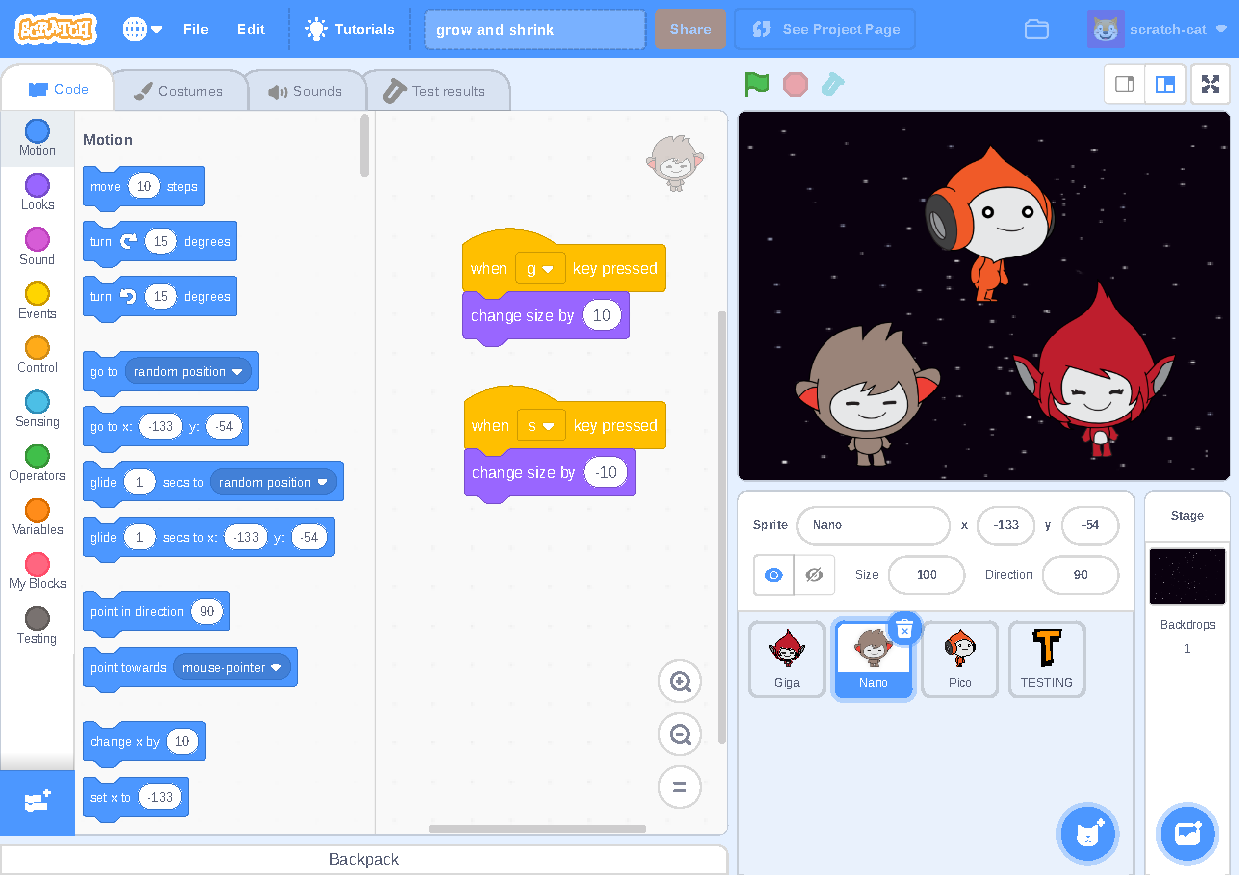
\includegraphics[width=\linewidth]{itch-grow-and-shrink-code}
    \end{wide}
    \caption{
        The \emph{Grow and shrink} exercise.
        A correct implementation of the exercise for the sprite \texttt{Nano} is seen here.
    }
    \label{fig:itch-grow-shrink-code}
\end{figure}

To illustrate Itch with a concrete example, we will use one exercise as a running example: the \emph{Grow and shrink} exercise (\cref{fig:itch-grow-shrink-code}).
In this exercise, there are three sprites: each sprite must grow if the \keys{g} key is pressed and must shrink if the \keys{s} key is pressed.
To test this exercise, we design a test suite that will verify the behaviour of the sprites (\cref{lst:grow-and-shrink-during}).
This test suite will:

\begin{enumerate}[noitemsep]
    \item Save the existing size of the sprites.
    \item Press the key that we are testing.
    \item Verify that the new size of the sprite is larger or smaller than the previously saved size.
    \item Save the new size as the existing size for the next test.
\end{enumerate}

\begin{listing}
    \begin{minted}{javascript}
function duringExecution(e) {
  const runtime = e.vm.runtime;
  // Save the original sizes of the sprites.
  const oldSize = {
    "Giga": runtime.getSpriteTargetByName("Giga").size,
    "Pico": runtime.getSpriteTargetByName("Pico").size,
    "Nano": runtime.getSpriteTargetByName("Nano").size
  }
  e.scheduler
    // Execute 4 events after each other.
   .forEach([1, 2, 3, 4], (prev) => {
     return prev.pressKey('g').log(() => {
       e.out.group("Test if sprites get bigger", () => {
         for (const sprite in oldSize) {
           const newSize = runtime.getSpriteTargetByName(sprite).size;
           e.out.test(`${sprite} got bigger`)
            .expect(newSize > oldSize[sprite])
            .toBe(true);
           // Save the new size as the old one.
           oldSize[sprite] = newSize;
         }
       })
     });
   }).forEach([1, 2, 3, 4], (prev) => {
    return prev.pressKey('s').log(() => {
      e.out.group("Test if sprites get smaller", () => {
        for (const sprite in oldSize) {
          const newSize = runtime.getSpriteTargetByName(sprite).size;
          e.out.test(`${sprite} got smaller`)
           .expect(newSize < oldSize[sprite])
           .toBe(true);
          oldSize[sprite] = newSize;
        }
      })
    });
  })
   .end();
}
    \end{minted}
    \caption{The complete test suite for the \emph{Grow and shrink} exercise in Itch.}
    \label{lst:grow-and-shrink-during}
\end{listing}

\section{Test suites}\label{sec:itch-test-suites}

Test suites for Itch are written in JavaScript.
A test suite for Itch is split into three phases:

\begin{enumerate}
    \item The \term{before execution} phase, which is run before the execution of the Scratch project.
    \item The \term{during execution} phase, where the test suite controls the Scratch project and simulates user interaction.
    \item The \term{after execution} phase, where tests are run on the log, which was collected during the previous phase.
\end{enumerate}

All phases are optional: it is perfectly valid to not have a before execution, or only a before execution, depending on the types of tests that need to be run.
They are implemented with ``magic'' functions: these have a fixed signature (name and arguments) and will be called in the relevant phases (\cref{lst:itch-test-suite-skeleton}).

\begin{listing}
    \begin{minted}{javascript}
/** @param {Evaluation} e */
function beforeExecution(e) {
    // Tests go here
}

/** @param {Evaluation} e */
function duringExecution(e) {
    // Tests go here
}

/** @param {Evaluation} e */
function afterExecution(e) {
    // Tests go here
}
    \end{minted}
    \caption[]{
        A skeleton of a test suite for Itch that shows the three phases.
        Each phase is implemented as a separate function that will be called at the appropriate time by Itch.
        The argument to these functions is an instance of the \mintinline{javascript}{Evaluation} class, which provides various methods to help with testing, such as the test structure, assertion functions, etc.
    }
    \label{lst:itch-test-suite-skeleton}
\end{listing}

Broadly, the tests can also be split according to their type: there are \term{static tests} and \term{dynamic tests}.
Static tests do not require execution of the Scratch project.
They are generally easier to write and faster to execute, but are severely limited in what they can test.
Assessing whether a project uses a certain block (e.g.\ a loop block) somewhere in the project is typically done with static tests.
Assessing whether a preprogrammed sprite (e.g.\ blocks that are provided in the starter project) was not modified is also done with static tests.
Static tests can be done completely in the before execution phase.

Checking more high-level goals, such as ``Does the sprite move when clicked?'', are more challenging with static tests.
At least, without severely limiting the accepted solutions.
For example, there are multiple ways to implement a sprite that moves when clicked, and a good behavioural test needs to accept all implementations.
For these kinds of behavioural tests, dynamic tests can be used, which require the project to be executed.
Dynamic tests often require both the during and the after execution phases.
In the during execution phase, user interaction is simulated and the behaviour is captured.
This captured behaviour can then be inspected in the after execution phase to see if the actual behaviour matches with the required behaviour.

Testing can also be done in the during execution phase, for example, after a user action has been performed.
While this makes some test suites easier (like the one in \cref{lst:grow-and-shrink-during}), it does require attention to the parallel nature of Scratch.
If multiple tests are run in parallel, the output can be garbled.

\subsection{Structure of a test suite}\label{subsec:structure-of-a-test-suite2}

A test suite consists of a hierarchical structure of groups and tests, which can be nested.
A test is a check on some requirement or property of the exercise.
It can be correct or wrong, and can contain feedback for both cases.
Additionally, a test also has a name and can include additional information, such as diffs, messages, etc.

Structure is added by grouping the tests.
Groups can be nested, so groups inside groups etc.\ are possible.
While there is no hard limit, the recommendation is to not go deeper than three levels in most cases.
Groups are used for more than just structure.
They also support a notion of visibility, with three modes:

\begin{itemize}[noitemsep]
    \item \emph{Visible}: the group is expanded (all children are visible).
    \item \emph{Hidden}: the group is completely hidden, unless one of the tests in the group fails.
    \item \emph{Summary}: the group is collapsed by default and a summary is shown unless one of the tests fails (in which case the group is expanded).
\end{itemize}

\begin{listing}
    \centering
    \begin{minted}{javascript}
        e.group.group('Tests for sprite A', () => {
          e.group
            .test('Sprite A does stuff right')
            .feedback({
              correct: 'Good job, sprite A does get stuff right!',
              wrong: 'Oh no, sprite A does not get it right.',
            })
           .expect('some value')
           .toBe('another value');
        });
    \end{minted}
    \caption{An example showing how the test suites are structured using groups and tests.}\label{lst:itch-test-suite-structure}
\end{listing}

Groups and tests in the JavaScript test suites are inspired by the Jest\footnote{\url{https://jestjs.io/}} testing framework.
The two relevant methods, \mintinline{javascript}{group} and \mintinline{javascript}{test} are available on the \mintinline{javascript}{Evaluation.group} property passed to the test suite.
\Cref{lst:itch-test-suite-structure} shows an example of this, containing a single test.
\marginnote{Maintainging backward compatibility is one of the downsides of using software in production.}
The double \mintinline{javascript}{group.group} is not a typo, but needed for backward compatibility with older test suites.
The test, as written in the example, will always fail, since it expects the string \mintinline{javascript}{"some value"} to be equal to \mintinline{javascript}{"another value"}.
The \mintinline{javascript}{expect}/\mintinline{javascript}{toBe} notation specifically will be familiar to Jest users.

Groups can be given just a name, as in the example, but it is also possible to provide more structured data.
For example, it is possible to link a group to a certain sprite.
This information is also provided in the generated feedback, which means the platform responsible for showing the feedback can, for example, show an image of the sprite with the group.

More details on how this structure is reflected in the generated feedback can be found in \cref{sec:format-of-the-generated-feedback}.
More metadata includes the visibility, a summary (used if the group's visibility is set to summary), some tags (which allows to tag groups with arbitrary strings), and an option to ignore wrong tests.
This last option means that if a test fails, it will be ignored completely and will not be outputted in the generated feedback.
This can be useful in cases where there are multiple possibilities: this allows trying each possibility until a passed test is found.

\subsection{Before execution}\label{subsec:before-execution}

The before execution phase allows for executing static tests.
Itch provides access to representations of two projects: the submission, created by the students, and the starter project, which is the project the students started with.

Providing both of these allows an easy way to assess whether the students modified some sprites or blocks in a sprite.
Itch provides helpers to ensure that students only modified certain sprites, or only certain code within sprites.
While this does limit the students in their ability to creatively modify the project, it makes behavioural tests for complex projects easier.
By limiting where the students are allowed to modify blocks, later tests can rely on certain functionality or sprites being available and working.
For example, if the project contains blocks that check if a sprite touches another sprite, these can be relied on.

This functionality of checking a set of predefined blocks and sprites is exposed with the function \mintinline{javascript}{Itch.checkPredefinedBlocks} to test suite authors.
For example:

\begin{minted}{javascript}
    Itch.checkPredefinedBlocks({
      spriteConfig: {
        SpriteA: script(whenIReceive('Start'), setEffectTo('ghost', 0)),
        SpriteB: {
          pattern: script(whenIReceive('Start'), setEffectTo('ghost', 0)),
          allowedBlocks: [forever()],
          allowAdditionalScripts: true,
        },
      },
      debug: false,
    }, e);
\end{minted}

The example above contains tests for two sprites.
All other sprites must be unchanged.

For the sprite \texttt{SpriteA}, students are allowed to change, add, or remove blocks in the script starting with the two blocks \scratchinline{\blockinit{when I receive \selectmenu{Start}}} and \scratchinline{\blocklook{set \selectmenu{ghost} effect to \ovalnum{0}}}.
Students are allowed to change blocks after these two predefined blocks.

The second sprite, \texttt{SpriteB}, allows modifications to scripts starting with the same blocks, but it uses the full version of the config object.
With the full version, it is also possible to specify if additional scripts are allowed and limit the blocks they can use.
In this example, only the \scratchinline{\blockinfloop{forever}{\blockspace[0.2]}} block can be used (so this is not a very useful test).
Finally, additional scripts (thus new ones created by the students) are also allowed.
These are free of restrictions: the check for allowed blocks does not apply.

\begin{listing}
    \begin{wide}
        \begin{subfigure}{0.49\linewidth}
            \begin{scratch}[scale=0.8]
                \blockinit{when I receive \selectmenu{Start}}
                \blocklook{set \selectmenu{ghost} effect to \ovalnum{0}}
                \blockrepeat{repeat \ovalnum{15}}
                {
                    \blocklook{change size by \ovalnum{3}}
                    \blockmove{change y by \ovalnum{-2}}
                }
                \blockrepeat{repeat \ovalnum{15}}
                {
                    \blocklook{change \selectmenu{ghost} effect by \ovalnum{5}}
                    \blockmove{change size by \ovalnum{3}}
                }
                \blocklook{hide}

            \end{scratch}
            \caption{A script in Scratch.}
        \end{subfigure}
        \begin{subfigure}{0.5\linewidth}
            \begin{minted}{javascript}
            script(
              whenIReceive('Start'),
              setEffectTo('ghost', 0),
              repeat(15, script(
                changeSizeBy(3),
                changeYBy(-2)
              )),
              repeat(20,script(
                changeEffectBy('ghost', 5),
                changeSizeBy(3)
              )),
              hide(),
            );
            \end{minted}
            \caption{The equivalent in JavaScript.}
        \end{subfigure}
    \end{wide}
    \caption{An example of how a Scratch program can be represented using the abstractions provided by Itch.}\label{lst:itch-block-abstraction}
\end{listing}

Itch also includes an abstraction to represent Scratch blocks in JavaScript, as used in the example above.
For each Scratch block, a corresponding function exists (see an example in \cref{lst:itch-block-abstraction}).

The functions representing blocks can also be used to construct block patterns.
Two additional functions are provided for patterns.
The first is \mintinline{javascript}{anything()}, which can be used in any location (as a block or value) and matches any block or value.
The reverse, \mintinline{javascript}{nothing()}, matches no block or value.
It can be useful to ensure that a script terminates (i.e.\ that there are no more blocks afterwards).
Additionally, an array of blocks or patterns can also be used in most places.
This represents a choice: it will match any of the patterns in the array.

For example, consider the following pattern:

\begin{minted}{javascript}
    repeat([15, 30], script(changeSizeBy(any()), never()))
\end{minted}

It will match a \scratchinline{\blockrepeat{repeat \ovalnum{}}{\blockspace[0.2]}} block that repeats 15 or 30 times, with a body with exactly one block, \scratchinline{\blocklook{change size by \ovalnum{}}}, whose argument can be anything.

Since scripts form a tree of blocks, there are also helpers to match and test against a script of blocks.
This supports error messages for each block (meaning they each show up as a failed assertion in the feedback).

\subsection{During execution}\label{subsec:during-execution}

\begin{listing}
    \begin{minted}{javascript}
        /** @param {Evaluation} e */
        function duringExecution(e) {
          e.scheduler
           .greenFlag(true)
           .wait(800)
           .pressKey('s')
           .end();
        }
    \end{minted}
    \caption{An example of the during execution phase where the scheduler is used to first press the green flag, wait \qty{800}{\milli\second}, press the \keys{s} key, and finally end execution.}\label{lst:itch-scheduler-example}
\end{listing}

The during execution phase is actually run just before the project is executed by Itch.
The main purpose of this phase is to use the \mintinline{javascript}{e.scheduler} (an instance of the \mintinline{javascript}{Scheduler} class) to schedule the execution of the project.
Using the scheduler, the test suite must specify how the project should be executed.
This includes starting execution, stopping execution, manipulating the virtual machine, and simulating user interaction, like clicking, key presses, input, and so on.
\Cref{lst:itch-scheduler-example} shows a minimal example of a schedule where the green flag is pressed, \qty{800}{\milli\second} must pass, and finally the \keys{s} key is pressed.

The scheduler receives a set of actions to perform.
Each next action is executed after the previous one has been scheduled or completed.
Because Scratch is a highly concurrent language, the scheduler also supports this.
First, most actions support a synchronous and asynchronous variant.
In the asynchronous variant, the action is executed and immediately finished.
For example, the action to press the green flag is almost instant: the green flag is pressed in the virtual machine, and the action is complete.

The synchronous actions will only finish after all activated scripts in Scratch have terminated.
For example, the action to press the green flag will wait on all scripts with the hat block \scratchinline{\blockinit{when \greenflag clicked}} are done executing.
Of course, there are scenarios where this is not possible.
If one of the scripts contains an infinite loop, the next scheduled action would never be performed, as the script will never end.

Since the project that is run comes from students with unknown code, synchronous actions also support a timeout.
After this time has passed, a failed assertion will be added to the generated feedback, and the scheduler will continue.

Every action in the scheduler returns the last scheduled action: this return value can be used to schedule a next action after the previous one.
To create a non-linear schedule (e.g.\ multiple actions are performed simultaneously), there are a few options.
First, the return value of one of the previous actions can be used multiple times to schedule new actions.
All of these will be run in parallel.

\begin{figure}
    \begin{subfigure}{0.49\linewidth}
        \centering
        \begin{minted}{javascript}
            const s = e.scheduler.wait(500);

            // Schedule actions L1-4
            s.forEach([1, 2, 3, 4], (p) => {
                return p.wait(500);
            });

            // Schedule actions N1-4
            s.forEach([1, 2, 3, 4], (p) => {
                p.wait(500);
                return p;
            });
        \end{minted}
    \end{subfigure}
    \begin{subfigure}{0.49\linewidth}
        \centering
        \includestandalone{itch-scheduler}
    \end{subfigure}
    \caption{
        The code for the scheduler (left) and the resulting schedule of actions (right).
        The start of an action is shown with a circle.
        After the start action S, the L and N actions are scheduled at the same time.
        However, the L actions return the new action in the function, meaning L1-4 will run sequentially.
        The code for the N actions returns the original action, meaning N1-4 will run in parallel.
        Since both N1 and L1 are scheduled on the same action S, the actions L1 and N1-4 will all run in parallel.
    }
    \label{fig:itch-scheduler-schedule}
\end{figure}

Another option is to use the method \mintinline{javascript}{forEach}: this is an implementation of the ``fold'' function on the events.
By deciding what action is used as the accumulator, either a linear (by returning the new action) or non-linear schedule (by returning the existing action) can be created.
\Cref{fig:itch-scheduler-schedule} shows an example of this.
By returning the new action, each action L1-4 will be performed in succession.
By returning the original action, the N1-4 actions will all be scheduled at the same time.
Since both L1 and N1 are scheduled on the same starting action S, they will also run in parallel.

While most actions are equivalent to their counter-parts in Scratch (like clicking a sprite, pressing a key, etc.), the wait action has more features.
In addition to waiting a set amount of time (like in the example), the wait action can also wait on the fulfillment of a certain condition.
The wait condition can be either waiting on a certain broadcast being sent, or a sprite fulfilling some condition.
The possible sprite conditions are moving, reaching a certain position, touching another sprite, no longer touching another sprite, touching the edge, and touching the mouse.
These conditions are added as needed, so with use, we envision more conditions being added.

A final special action is the \mintinline{javascript}{log} action.
This action saves the current state in the log (\cref{subsec:after-execution}) and executes a custom function at that time.
This action is intended to mark certain events in the log, but can also be used to execute a test during the execution of the project, instead of beforehand or afterwards.
While the test is executed during the execution, it also has access to snapshots and events that have already taken place.

\subsection{After execution}\label{subsec:after-execution}

\begin{listing}
    \begin{minted}{javascript}
        function duringExecution(e) {
          // Schedule pressing each key four times in succession.
          e.scheduler
           .forEach([1, 2, 3, 4], (prev) => prev.pressKey('g'))
           .forEach([1, 2, 3, 4], (prev) => prev.pressKey('s'))
           .end();
        }

        function afterExecution(e) {
          const sprites = ["Giga", "Pico", "Nano"];

          // Get the events for the g key presses.
          const gPresses = e.log.events.filter((e) => e.type === 'key' && e.data.key === 'g');
          for (const event of gPresses) {
            e.out.group("Test if sprites get bigger", () => {
              for (const name of sprites) {
                // Get the sprite from the snapshot before the key press.
                const before = event.previous.sprite(name);
                // Get the sprite from the snapshot after the key press.
                const after = event.next.sprite(name);

                e.out.test(`${name} got bigger`)
                 .expect(after.size > before.size)
                 .toBe(true);
              }
            });
          }

          const sPresses = e.log.events.filter((e) => e.type === 'key' && e.data.key === 's');
          for (const event of sPresses) {
            e.out.group("Test if sprites get smaller", () => {
              for (const name of sprites) {
                const before = event.previous.sprite(name);
                const after = event.next.sprite(name);

                e.out.test(`${name} got smaller`)
                 .expect(after.size < before.size)
                 .toBe(true);
              }
            });
          }
        }
    \end{minted}
    \caption{
        Alternative test suite for the \emph{Grow and shrink} exercise.
        In contrast to \cref{lst:grow-and-shrink-during}, this test suite only schedules the key presses in the during execution phase.
        All tests after performed in the after execution phase using the log.
    }
    \label{lst:grow-and-shrink-after}
\end{listing}

Itch uses the scheduler from the during execution phase to execute the submission.
During the execution, a log is constructed of the execution.
This is done by hand (using the \mintinline{javascript}{log} scheduler action) and automatically at interesting points.
The log consists of snapshots (which are taken every time something changes in the virtual machine) and events (which denote interesting snapshots).
For example, every action in the scheduler is saved as an event, meaning there is a snapshot before the action and after the action has been completed.

Returning to the \emph{Grow and shrink} exercise, \cref{lst:grow-and-shrink-after} shows an alternative test suite (compared to \cref{lst:grow-and-shrink-during}).
In the during execution phase, only the key presses are scheduled.
Afterwards, in the after execution phase, the log is used to perform the tests.
For each key press, the corresponding event in the log is looked up.
Each of these events provides before and after snapshots, which are then used to determine if sprites correctly change in size.

\section{Evaluating projects}\label{sec:itch-evaluating-projects}

The evaluation of a submission goes through the following process:

\begin{enumerate}
    \item The submission, the starter project, and the test suite are made available.
    \item Itch loads both projects, and runs the before execution phase.
        While the starter project is available in all phases, it is only intended to be used in the before execution phase.
    \item If the before execution phase does not result in an error, Itch initialises the virtual machine, inserts hooks for the log, and loads the submission into the virtual machine.
    \item The during execution phase is run, and the scheduled actions are read from the test suite.
        The during execution phase is used to create a schedule of user actions using the scheduler.
        It does not actually run the schedule itself.
    \item Itch starts the virtual machine and executes the scheduled actions.
          While executing, the logs are captured.
    \item If the execution does not result in an error, Itch shuts down the virtual machine, and runs the after execution phase.
    \item All feedback is sent to the output.
        The output is a callback function that can be provided when starting Itch, or the default function is used, which prints the feedback on standard output.
\end{enumerate}

Scratch 3.0 is built using browser technologies, and has to be run in the browser.
While the virtual machine is pure JavaScript and could thus run without a browser, the renderer is not: it uses the HTML canvas and WebGL technologies.
The renderer is used to calculate things like sprite collisions and checking if sprites touch certain colours.
While it is theoretically possible to create a renderer that does not use WebGL, this would be a big undertaking and imply a big maintenance burden.
The re-implemented renderer will have to be kept up to date with the upstream one and replicate all behaviour exactly.

Itch consists of two JavaScript packages, which is a reflection of the two ways to run Itch:

\begin{itemize}
    \item As a library in the browser.
          This is useful for contexts where there already is a browser, e.g.\ running Itch along the Scratch environment on the device of the student for client-side testing.
        This is implemented by the first JavaScript package, the core package.
    \item As a command line tool.
          This is for cases where Itch runs as a service in the backend, e.g.\ to check submissions after students are done.
        This is implemented in the second JavaScript package, the runner package.
        This package wraps around the core package to launch the browser instance and load the various dependencies (it thus runs the core package, which is where it gets its name).
\end{itemize}

\subsection{Running Itch as a library}\label{subsec:running-itch-as-a-library}

\begin{listing}
    \begin{minted}{typescript}
        export interface EvalConfig {
          /** The submission sb3 data. */
          submission: ArrayBuffer;
          /** The starter project sb3 file. */
          template: ArrayBuffer;
          /** If the output should be partial or full. */
          fullFormat: boolean;
          /* The canvas for the renderer. */
          canvas: HTMLCanvasElement;
          /** The test suite to use. */
          testplan: string | TestplanSource;
          /** Callback for the results. */
          callback: OutputHandler;
          /** The language of the exercise. */
          language: string;
        }

        /** Run the judge. */
        export async function run(config: EvalConfig): Promise<void>;
    \end{minted}
    \caption{The exposed interface to run Itch. It consists of one function and a configuration object.}\label{lst:itch-library-interface}
\end{listing}

When running Itch as a library, the core package must be loaded into the browser, in addition to having the Scratch dependencies (the virtual machine, etc.) available.
The exposed interface to run Itch is limited to one function and a configuration object (\cref{lst:itch-library-interface}).
Most of the options are self-explanatory, and the output format option is explained in \cref{sec:format-of-the-generated-feedback}.

\subsection{Running Itch as a command line tool}\label{subsec:running-itch-as-a-command-line-tool}

\begin{figure}
    \begin{wide}
        \includestandalone[width=\linewidth]{itch-sequence-diagram}
    \end{wide}
    \caption{Sequence diagram showing the process of evaluating a project with Itch. When run as a library, there is no itch core or Puppeteer.}
    \label{fig:itch-sequence-diagram}
\end{figure}

When there is no existing browser instance  available, Itch provides a command line interface.
\marginnote{A headless browser is a full browser, but without user interface.}
In this mode, Itch will run a headless browser, load the projects and test suites, run the judge, and finally collect the results from the browser.
\Cref{fig:itch-sequence-diagram} shows the complete process.

First, the runner package launches a Puppeteer instance.
After it is read, the various dependencies are loaded into the Puppeteer instance (these are the Itch core package, the Scratch dependencies, the test suite, the submission, and the starter project).
The runner package will then run a special script that will call Itch as it would be used as a library: the \mintinline{typescript}{run(config)} function is called.
Then, the same process happens as when using Itch as a library.
First, the projects (submission and starter) are parsed.
The phases are then executed, with the before and during execution phase going first.
The during execution phase results in a schedule, which is then run.
The virtual machine is started and runs the projects with the scheduled actions.
Finally, the after execution phase is run, with the log from the previous phase.

\subsection{Performance considerations}\label{subsec:performance-considerations}

Reducing the time students spend waiting on feedback is essential for providing a good user experience with software testing, especially in educational software testing~\autocite{sarsaSpeedingAutomatedAssessment2022}.
One difficulty in providing fast feedback on Scratch code is that blocks that wait are commonly used.
However, these wait times pose a hard lower limit on the duration of the evaluation of a Scratch project.
For example, if a project has a wait block for 2 seconds, the evaluation time of said project can never be less than 2 seconds (and will be higher in practice, since the whole evaluation process also adds overhead).
Such wait blocks can quickly add up.

As a solution for this problem, Itch provides test suites with the ability to set an ``acceleration factor'': this factor indicates the speedup for all time-based data, both in the project and in the test suite.
For example, if the acceleration factor is 2, the wait time in wait blocks will be halved, as will wait times in the scheduler.
The acceleration factor can, however, be flaky with high values: we do not recommend a factor higher than 5.
If it is expected that, for example, wait blocks are used for synchronization of two sprites, the acceleration factor can cause issues, as it does not speed up general execution.

Itch also provides the test suite with the possibility to enable Scratch's built-in turbo mode.
In this mode, execution is done faster (how much depends on the project).
Together with the acceleration factor, these techniques can significantly speed up the evaluation.

\section{Format of the generated feedback}\label{sec:format-of-the-generated-feedback}

The format of the generated feedback is in structure very similar to the structure of the tests in the test suite (\cref{subsec:structure-of-a-test-suite}).
The three levels of the feedback are:

\begin{itemize}[nosep]
    \item \term{Judgement}: the top-level object of the feedback.
    \item \term{Group}: contains one or more tests or subgroups (equivalent to a group from the test suite).
        Each group has the same options as in the test suite (e.g.\ visibility, sprites).
    \item \term{Test}: one condition or requirement that is evaluated (equivalent to a test from the test suite).
\end{itemize}

When running Itch as a library, it is possible to provide a callback function that will be called when feedback is available.
There are two modes for this: the partial mode or the full mode.
In the partial feedback mode, feedback is streamed to the callback: it is called whenever feedback is available.
In the full mode, the callback is called once at the end with a fully constructed feedback object that contains all feedback for the evaluation.

When running Itch on the command line, the feedback is outputted to the standard output stream (this is also possible when using Itch as a library).
Depending on the feedback mode, the format is slightly different.

\begin{listing}
    \begin{minted}{json}
        {"command": "start-judgement", "version": 2}
        {"command": "start-group", "name": "Check on existing code", "visibility": "summary"}
        {"command": "start-group", "name": "Stage", "sprite": "Stage", "visibility": "summary"}
        {"command": "start-test", "name": "Sprite exists"}
        {"command": "close-test", "feedback": "The sprite exists", "status": "correct"}
        {"command": "close-group"}
        {"command": "close-group"}
        {"command": "close-judgement"}
    \end{minted}
    \caption{Example of the output generated by Itch for a test suite with two nested groups, with one test. Note the similarity to \cref{lst:tested-output-example}.}\label{lst:itch-output-example-partial}
\end{listing}

The partial feedback format is very similar to the Dodona feedback format used by TESTed (\cref{subsec:dodona-output}).
An example of this feedback is given in \cref{lst:itch-output-example-partial}.
The format is newline-delimited JSON: JSON objects are separated by a newline, and each line is a valid JSON object.
The structure of the feedback is indicated by commands, with \texttt{start} commands to begin a new level in the hierarchy and \texttt{close} commands to finish a level.

In full feedback mode, the output is a single JSON object that represents a nested tree of the same feedback.

\section{Itch in practice}\label{sec:itch-evaluation}

In this section, we discuss the use of Itch in educational practice, and discuss insights from creating test suites for Scratch exercises.

\subsection{Capabilities of the testing framework}\label{subsec:capabilities-of-the-testing-framework}

The initial development of Itch used a set of 13 Scratch exercises from the 2017 edition of the Flemish Programming Contest (\textdutch{\emph{Vlaamse Programmeerwedstrijd}}).
The Scratch exercises were used in a special category for students aged 10 to 12.
This category was a one-time event organized by the local organizer as a side-event for the Programming Contest, which normally focuses on text-based programming languages.
It is worth mentioning that this event used human judges to assess whether the children had successfully completed an assignment.
This was the case as there were no Scratch testing frameworks at the time that could automate this assessment: as a result, the exercises were not created with automated assessment in mind.

These 13 exercises were used as a reference for the initial feature set and capabilities of Itch.
The exercises can be classified into five groups, depending on their contents:

\begin{description}
    \item[Speaking] Sprites speak, think, or ask questions (5 exercises).
    \item[Moving] Sprites move around (3 exercises).
    \item[Costumes] Sprites change costumes, often to emulate animation (3 exercises).
    \item[Games] Interactive games that require user input (1 exercise).
    \item[Drawing] The \emph{Pen} extension is used to draw on the canvas (3 exercises).
\end{description}

Note that the exercises do not sum up to 13: two exercises are both in the moving and costumes category, since they do both.

For 12 of the 13 exercises, an Itch test suite was created that tested the submissions sufficiently that it would have been usable in the programming contest.
The remaining exercise was not testable due to its open-ended nature.
This exercises boils down to ``draw a house'', which results in a vast variety of houses.
Besides introducing some computer vision framework to detect houses (which is technically possible in Itch), this is not easily testable.

These exercises were all tested with dynamic tests, meaning they test the behaviour of the submission.
The exercises of CodeCosmos (which are discussed in \cref{subsec:itch-in-educational-practice}) are often longer interactive games.
Due to their complex nature, static testing was sometimes needed (which is discussed in \cref{subsec:creating-test-suites-for-scratch-exercises}).

\subsection{Itch in educational practice}\label{subsec:itch-in-educational-practice}

At a later point in the development of Itch, it has been used in educational practice.
This was mainly done by our partner, CodeCosmos.
CodeCosmos provides the platform in which Itch is integrated.
The platform provides a variety of organizational tools, like classroom management.
Specially for Scratch, the platform has its own hosted instance of the Scratch environment (similar to the \textsc{mit}-hosted instance).
This instance has been modified to integrate with Itch.

In the platform, Itch is run server-side by a dedicated service.
The choice for server-side testing versus client-side testing was mainly motivated by making sure that students could not cheat by modifying the test suites or the results.
The platform will periodically (or when a button is pressed) send the current version of the submission to the server.
The backend will then look up the test suite and starter project and send these to the Itch service.
After testing has been completed, the results are returned to the platform where they are displayed to the students in an additional, custom tab in the Scratch environment.

There are two different ways in which the CodeCosmos programming exercises are used.
The first is as part of a ``teaching pack'', which is bought and used by schools.
These packs implement the ``attainment descriptors''\marginnote{Called \textenglish{eindtermen} in Dutch.}, which are documents that describe the learning objectives of the lessons and what skills students should possess after taking the courses.
Here, the teaching pack provides a full learning path for the students, with suitable exercises at each stage of the process.
The second way is as an extracurricular activity, where students either follow weekly lessons or join a ``coding camp'' for a few weeks in the summer.
In both cases, many of the same exercises are used, but the context in which they are used differs.

In total, there are 139 exercises with an Itch test suite.
In the period from March 3rd, 2023 until March 26th, 2024 (328 days), Itch evaluated \num{28144} submissions.
Of these submissions, \num{2713} (\qty{9.64}{\percent}) are evaluated as being correct, which means \qty{90.36}{\percent} of evaluated submissions are incorrect.
This is in line with our expectations: we allow students to submit as much as they want (and even automatically submit every so often) until the submission is correct.
This also allows for collecting information about the trajectory of students while solving an exercise, but also provides more data for analysing the growth of students throughout a course.
Providing insights from this data to educators is one area of future work that is planned by CodeCosmos.

The submissions were made by \num{6496} unique users, with an average of \num{4.33} submissions per user.
The submissions have an average test count of \num{158}, (the exercises have a number of tests that range from a minimum of \num{2} and a maximum of \num{1292}).

Most of these exercises were conceived before introducing Itch, meaning Itch is capable of evaluating exercises as typically used by CodeCosmos.
The biggest change we made to the exercises was splitting the levels of the exercises into different Scratch projects.

\subsection{How to assess Scratch submissions}\label{subsec:how-to-evaluate-scratch-submissions}

The creators of Scratch have a well-known vision on how they intend Scratch to be used.
Generally, the Scratch team prefers not to use assignment-based learning~\autocite{resnickCodingCrossroads2020}.
As a specific example of this, they particularly do not support strict static tests on exercises.
For example, they express this as follows in~\autocite{resnickCodingCrossroads2020}:

\begin{quotation}
    Too often, researchers and educators are adopting automated assessment tools that evaluate student programming projects only by analyzing the code, without considering the project goals, content, design, interface, usability, or documentation.
    \marginnote{They are probably talking about Dr.\ Scratch here.}
    For example, many are using an online Scratch assessment tool that gives students a ``computational thinking score'' based on the assumption that code with more types of programming blocks is an indication of more advanced computational thinking.
    This form of assessment doesn't take into consideration what the student's program is intended to do, how well it accomplishes the student's goals, whether the code works as intended, whether people are able to interact with it, or how the student's thinking develops over a series of projects.
\end{quotation}

At the same time, using linters or other static analysis tools to detect code smells is beneficial for students~\autocite{hermansCodeSmellsHamper2016}.
However, in Itch, static analysis can also be used for automatic assessment by writing the static tests in the before execution phase of the test suite.
While we share the sentiment of \citeauthor{resnickCodingCrossroads2020}, our experience with Scratch exercises and our collaboration with CodeCosmos has shown that such tests are often used, despite their disadvantages.
There are a few factors that contribute to this:

\begin{itemize}
    \item Exercises (especially in Scratch) that were not created with testability in mind are hard to properly test without resorting to static analysis of the code.
    \item Scratch projects, especially complex ones, are technically challenging to test within an acceptable time frame.
        We cannot spend minutes evaluating a single submission, as feedback must be provided quickly to students~\autocite{sarsaSpeedingAutomatedAssessment2022}.
    \item Educators want simple metrics to easily see if students have mastered some concept.
          For example, determining if a student has mastered the concepts of loops (or repetition in general) is challenging to do automatically.
          With a large number of students and time constraints, educators fall back on analyzing blocks as a proxy for mastery~\autocite{combefisAutomatedCodeAssessment2022}.
\end{itemize}

This does not mean that static tests are of no use: with good and thoughtful static tests, an educator (and student) can be fairly certain that a submission marked as correct is effectively correct.
This can guide the educator to spend more time on submissions where their attention is warranted.
Similarly, a submission marked as wrong can also help pinpoint the problem to the student, without intervention from the educator.

However, as so eloquently stated by Edsger Dijkstra, ``Testing shows the presence, not the absence of bugs''.
Students might have solved the exercise in creative or innovative ways, which static tests fail to detect.
Similarly, they might have fooled the static tests into marking the submission as correct, even though it is not.
Therefore, we do not recommend using static tests to automatically grade submissions, at least not without verifying the results.

\subsection{Creating test suites for Scratch exercises}\label{subsec:creating-test-suites-for-scratch-exercises}

Itch does not use the same programming language for the test suites as the programming language of a submission: test suites for Scratch exercises are written in JavaScript.
\marginnote{Doing the same in Scratch would be much less ergonomic then doing it in JavaScript.}
While this has advantages, as JavaScript is a general purpose programming language, while Scratch is much more limited, it also has disadvantages.

It is not uncommon for educators that use or create Scratch exercises to have no formal computer science background, nor experience with programming besides Scratch~\autocite{kimEnhancingTeachersICT2012,oliveiraIntroductionComputationalThinking2019}.
This is also the case at CodeCosmos, where teachers with an educational background design and create the exercises.
For the existing exercises, the educators designed the exercise and implemented the Scratch parts, while others (like the author) with more experience with JavaScript, implemented the test suites.
However, it is our experience that it is faster if the people designing the exercise have knowledge of the testing framework and implement the test suite themselves.
In \cref{sec:poke:-a-testing-framework-written-in-scratch}, we explore an experiment showing what a testing framework for Scratch with test suites in Scratch may look like.

\section{Writing test suites in Scratch}\label{sec:poke:-a-testing-framework-written-in-scratch}

As mentioned in the previous subsection, creating test suites in JavaScript for Scratch exercises can be challenging for educators without computer science background or experience.
To fill this gap, we have developed Poke: a prototype of a testing framework for Scratch implemented in Scratch itself.
This means that test suites are written with Scratch blocks, tests are executed in the Scratch environment, and the results are also shown in the Scratch environment.

For this prototype, our focus was on two research questions: ``Is it possible to create a testing framework for Scratch in Scratch?'' and ``If possible, which testing facilities should be present?''.
The answer to the first question is yes, and the remainder of this section discusses the details of Poke, along with answers for the second question.
These considerations include what blocks to provide, how tests should be run, etc.

\subsection{Introduction to Poke}\label{subsec:introduction-to-poke}

\begin{figure}
    \begin{wide}
        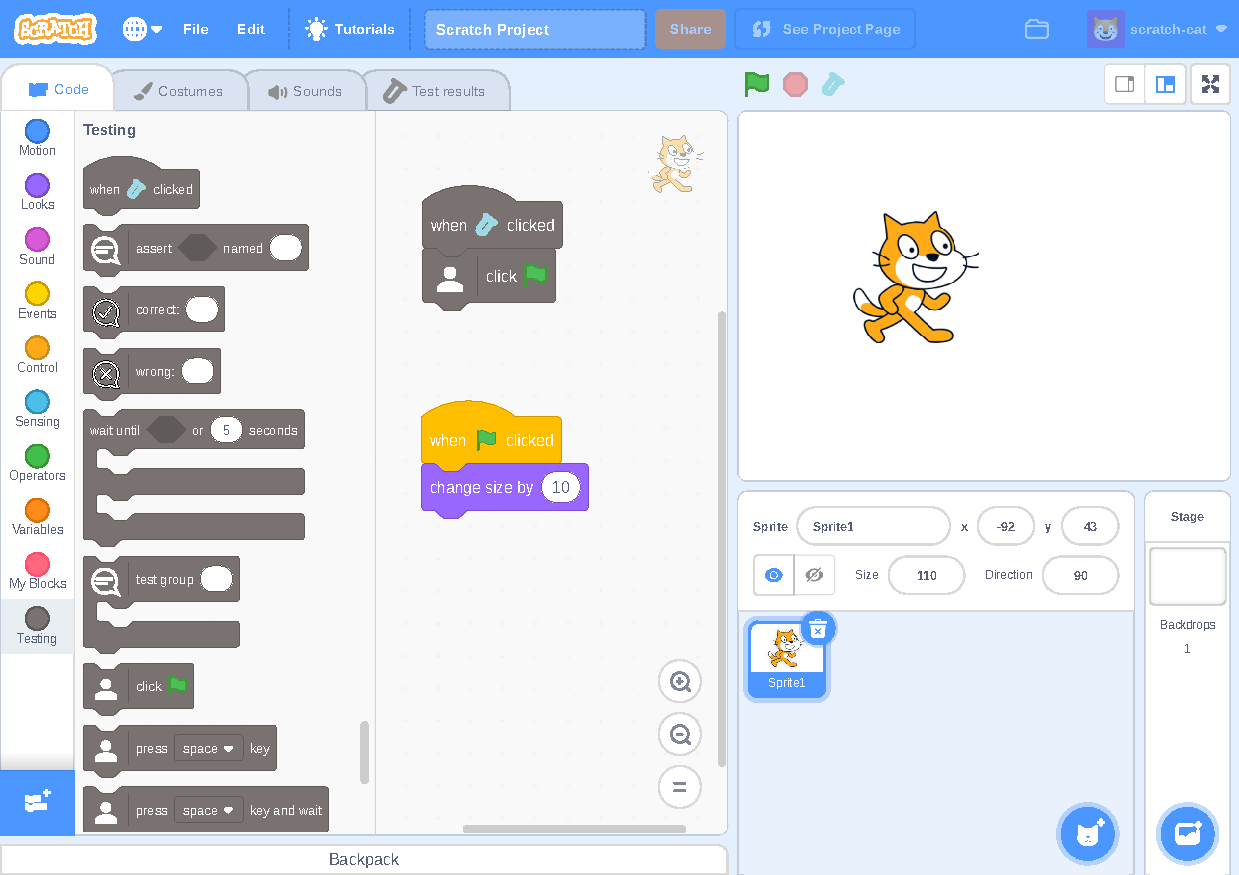
\includegraphics[width=\linewidth]{poke-ui}
    \end{wide}
    \caption{The Scratch environment with the added Poke elements: the additional button next to green flag and stop buttons to start the tests, the additional tab to show test results, and the extension that provides the Poke blocks.}
    \label{fig:poke-ui}
\end{figure}

The user-facing part of the Poke software testing framework consists of three parts (\cref{fig:poke-ui}):

\begin{itemize}
    \item An additional button next to the green flag and stop button, which will run the tests.
    \item An extension to provide a set of blocks to write tests with.
    \item An additional tab in the Scratch environment that shows the test results once run.
\end{itemize}

\subsection{The Poke extension}\label{subsec:poke-provided-blocks}

Poke provides five categories of blocks: a hat block (\scratchinline{\blockpokehat{when \drawtesttube clicked}}, which starts the tests if the button is clicked), feedback blocks, user interaction blocks, observation blocks, and blocks to execute code in another sprite.

\subsubsection{Feedback blocks}

\begin{scratch}[scale=0.6]
    \blockpokegroup{\drawicon{\drawfeedback} test group \ovalnum{name}}{\blockspace[0.5]}
\end{scratch}

The structure of a test suite in Poke is identical to the structure in Itch (\cref{subsec:structure-of-a-test-suite2}): a test suite consists of groups, which can contain tests or other groups.
The block for creating groups is a C block that takes the name of the group as an argument.
The body of the block outputs its test results in the group.

\begin{wide}
    \begin{varwidth}{0.40\linewidth}
        \begin{scratch}[scale=0.6]
            \blockpoke{\drawicon{\drawfeedback} assert \boolpokeempty[3em] named \ovalnum{feedback}}
        \end{scratch}
    \end{varwidth}%
    \hspace{1em}%
    \begin{varwidth}{0.28\linewidth}
        \begin{scratch}[scale=0.6]
            \blockpoke{\drawicon{\drawfeedbackcorrect} correct: \ovalnum{feedback}}
        \end{scratch}
    \end{varwidth}%
    \hspace{1em}%
    \begin{varwidth}{0.25\linewidth}
        \begin{scratch}[scale=0.6]
            \blockpoke{\drawicon{\drawfeedbackwrong} wrong: \ovalnum{feedback}}
        \end{scratch}
    \end{varwidth}
\end{wide}

For generating test results, there are three blocks, the main of which is the assertion block.
It takes a boolean value and a name.
The name is shown in the output, together with a status depending on the value of the boolean block.
There are also the correct and wrong blocks, which act as a test that always passes or always fails respectively.

\begin{scratch}[scale=0.6,else word={}]
    \blockpokedgroup{\drawicon{\drawfeedback} wait until \boolpokeempty[3em] or \ovalnum{} seconds}{\blockspace[0.5]}{\blockspace[0.5]}
\end{scratch}

A special block is the wait until or timeout block.
This block will wait until the condition evaluates to true or the specified number of seconds has passed.
If the condition evaluates to true within the time limit, the first slot is used, which will often contain a \scratchinline{\blockpoke{\drawicon{\drawfeedbackcorrect} correct: \ovalnum{}}} block.
Otherwise, the second slot is used, which will often contain a \scratchinline{\blockpoke{\drawicon{\drawfeedbackwrong} wrong: \ovalnum{}}} block.
The two slots can also contain other blocks.

\subsubsection{User interaction blocks}

\begin{varwidth}{0.20\linewidth}
    \begin{scratch}[scale=0.6]
        \blockpoke{\drawicon{\drawinteract} click \greenflag}
    \end{scratch}
\end{varwidth}%
\hspace{1em}%
\begin{varwidth}{0.28\linewidth}
    \begin{scratch}[scale=0.6]
        \blockpoke{\drawicon{\drawinteract} click \selectmenu{Sprite}}
    \end{scratch}
\end{varwidth}%
\hspace{1em}%
\begin{varwidth}{0.3\linewidth}
    \begin{scratch}[scale=0.6]
        \blockpoke{\drawicon{\drawinteract} click \selectmenu{Sprite} and wait}
    \end{scratch}
\end{varwidth}

\begin{varwidth}{0.5\linewidth}
    \begin{scratch}[scale=0.6]
        \blockpoke{\drawicon{\drawinteract} press \selectmenu{space} key}
    \end{scratch}
\end{varwidth}%
\hspace{1em}%
\begin{varwidth}{0.5\linewidth}
    \begin{scratch}[scale=0.6]
        \blockpoke{\drawicon{\drawinteract} press \selectmenu{space} key and wait}
    \end{scratch}
\end{varwidth}%

\begin{varwidth}{0.5\linewidth}
    \begin{scratch}[scale=0.6]
        \blockpoke{\drawicon{\drawinteract} move mouse to x: \ovalnum{} y: \ovalnum{}}
    \end{scratch}
\end{varwidth}%
\hspace{1em}%
\begin{varwidth}{0.5\linewidth}
    \begin{scratch}[scale=0.6]
        \blockpoke{\drawicon{\drawinteract} answer \ovalnum{answer text}}
    \end{scratch}
\end{varwidth}%

The user interaction blocks will simulate user interaction, similar to the scheduler in Itch (\cref{subsec:during-execution}).
Currently, there are blocks to click the green flag, click a sprite, move the mouse, press a key, and answer a question.
The block to click a sprite and the block to press a key also have a synchronous variant, which will wait until all activated scripts have finished, again similar to the synchronous/asynchronous actions in the scheduler from Itch.

\subsubsection{Observation blocks}

\begin{varwidth}{0.2\linewidth}
    \setscratch{scale=0.6}\ovalpoke{\drawicon{\drawobserve} snapshot}
\end{varwidth}%
\hspace{1em}%
\begin{varwidth}{0.5\linewidth}
    \setscratch{scale=0.6}\ovalpoke{\drawicon{\drawobserve} \selectmenu{property} of \selectmenu{Sprite} in \ovalnum{snapshot}}
\end{varwidth}%
\hspace{1em}%
\begin{varwidth}{0.3\linewidth}
    \setscratch{scale=0.6}\ovalpoke{\drawicon{\drawobserve} \selectmenu{property} in \ovalnum{snapshot}}
\end{varwidth}

The observation blocks are very similar to sensing blocks from Scratch, as they allow the tests to save and query the environment.
A special sensing block (which also acts as a variable) reflects the current state of the virtual machine.
Test code can then save this state into a variable, making it available later.
Two more reporter blocks (one for sprite-specific properties and one for the stage) allow querying specific properties (of specific sprites) from the saved state (or the current state).

\subsubsection{Executing blocks in another sprite}

\begin{varwidth}{0.5\linewidth}
    \begin{scratch}[scale=0.6]
        \blockpokegroup{\drawicon{\drawsquarearrow} with \selectmenu{Sprite} do}{\blockspace[0.5]}{}
    \end{scratch}
\end{varwidth}%
\hspace{1em}%
\begin{varwidth}{0.5\linewidth}
    \begin{scratch}[scale=0.6]
        \blockpoke{\drawicon{\drawsquarearrow} add sprites to \selectmenu{list} where \boolpokeempty[3em]}
    \end{scratch}
\end{varwidth}%

While the test blocks can be placed in any sprite, it is our experience that the most convenient place is a dedicated sprite with only test code or in the stage if it does not have code itself.
However, this introduces an additional complication: how can the test sprite execute blocks in other sprites?
For example, the test sprite might want to move a certain sprite, which is not possible in vanilla Scratch.

To this end, Poke provides a C block, whose contents will be executed in the selected sprite.
Technically, this re-uses the broadcasting mechanism built into Scratch.
Behind the scenes, the following process happens:

\begin{enumerate}
    \item Before executing a test, Poke will generate a unique broadcast for each of these C blocks.
    \item The contents of the C block are copied to the sprite that will execute them.
    \item These copied blocks are placed under a hat block that will trigger when the generated broadcast is sent.
    \item The original blocks are replaced with a send broadcast block.
\end{enumerate}

When the virtual machine executes this code, it will send the broadcast, which will trigger the blocks in the correct sprite.
This happens transparently for the user: the copied blocks are not visible to the user, and special care has been taken to ensure that there are no performance issues.
For example, the blocks are only copied once (or when they are changed).

\subsection{Feedback in the Scratch environment}\label{subsec:feedback-in-the-scratch-environment}

% TODO: update Scratch environment?
% TODO: update icons to be svg...
\begin{figure}
    \begin{wide}
        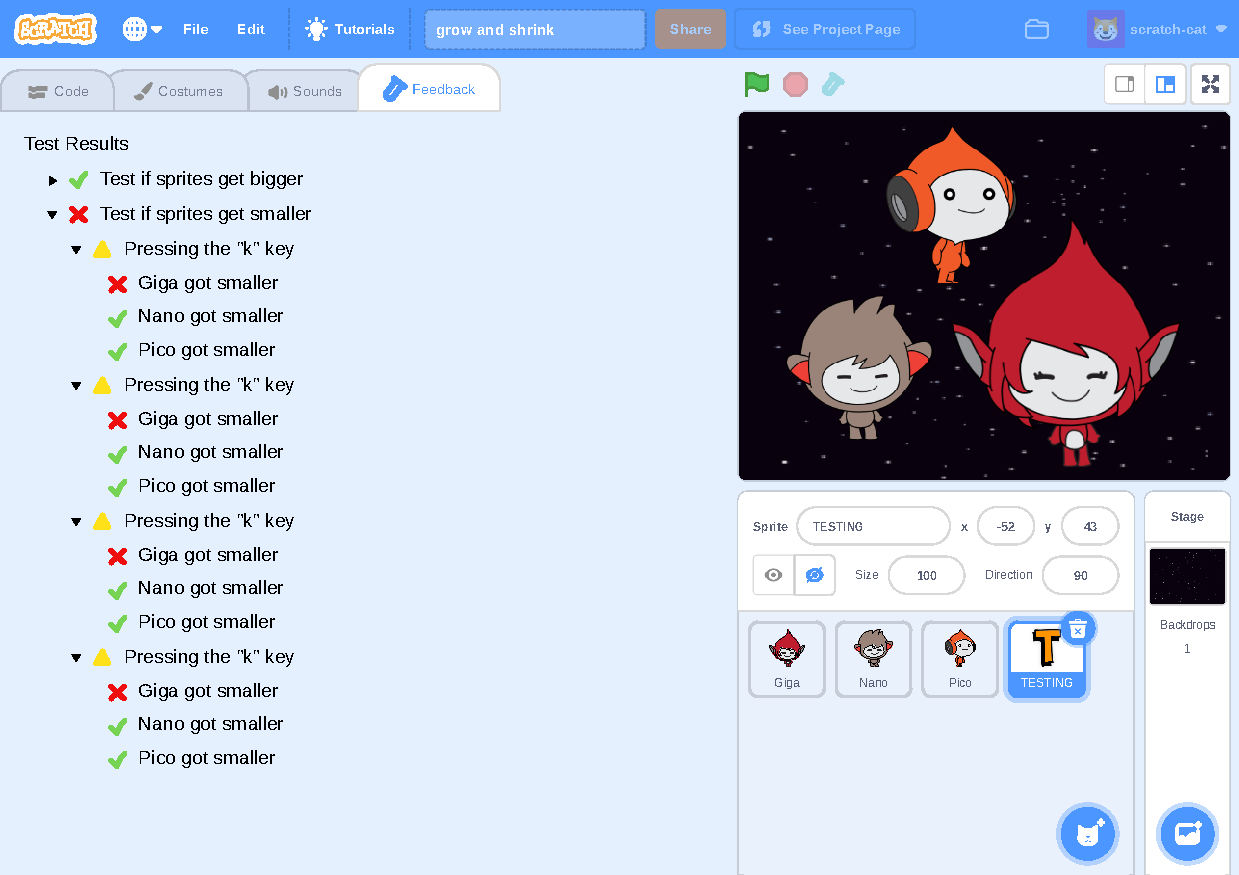
\includegraphics[width=\linewidth]{scratch-poke-feedback}
    \end{wide}
    \caption{
        Feedback for the \emph{Grow and shrink} exercise.
        The submission's implementation contains an error: the sprite \texttt{Giga} does not implement the shrinking behaviour (with the \keys{s} key).
        In the feedback, there are two test groups: one for checking that sprites grow and one for checking that sprites shrink.
        In each of these groups, the relevant key is pressed four times and each sprite is checked.
        In the ``grow'' group, everything is correct (indicated by the green checkmarks).
        As expected, the second group reports that some tests have failed (indicated by the yellow triangles).
        Two of the subgroups are open: while the tests for \texttt{Nano} and \texttt{Pico} were correct, the one for \texttt{Giga} failed as expected (indicated by a red crosses).
    }
    \label{fig:poke-feedback-result}
\end{figure}

For this prototype, showing feedback to students was not a priority.
As such, the feedback is shown in a rudimentary interface, which shows the feedback in a tree format (\cref{fig:poke-feedback-result}).
While usable, it is not the most intuitive layout, especially considering the target demographic of Scratch users.

\subsection{Comparing Poke to Itch}\label{subsec:comparing-poke-to-itch}

To verify that Poke is usable as a testing framework, we compared it to the set of Scratch problems from the Flemish Programming Contest (\cref{subsec:capabilities-of-the-testing-framework}) that were testable by Itch.

Three of the exercises could not be tested with Poke, but this was expected.
Poke does not support extensions at the moment, and these exercises use the pen extension.
One of these three exercises would not be testable anyway, for the same reason Itch could not test it: drawing a house is a very open-ended exercise.
The other exercises could be tested with Poke, if the pen extension were supported.

For comparison, \cref{lst:grow-and-shrink-during} contains the test suite for the \emph{Grow and shrink} exercise in Itch, while \cref{lst:poke-grow-and-shrink} contains the test suite used in Poke.

\begin{listing}
    \begin{wide}
    \begin{scratch}[scale=0.6]
        \blockpokehat{when \drawtesttube clicked}
        \blockpokegroup{\drawicon{\drawfeedback} test group \ovalnum{Test if sprites get bigger}}{
            \blockrepeat{repeat \ovalnum{4}}{
                \blockpokegroup{\drawicon{\drawfeedback} test group \ovalnum{Pressing the ``g'' key}}{
                    \blockvariable{set \selectmenu{snapshot-before} to \ovalpoke{\drawicon{\drawobserve} snapshot}}
                    \blockpoke{\drawicon{\drawinteract} press \selectmenu{g} key and wait}
                    \blockpoke{\drawicon{\drawfeedback} assert \booloperator{\boolsensing{\selectmenu{size} of \selectmenu{Giga}} > \ovalpoke{\drawicon{\drawobserve} \selectmenu{size} of \selectmenu{Giga} in \ovalvariable{snapshot-before}}} named \ovalnum{Gigga got bigger}}
                    \blockpoke{\drawicon{\drawfeedback} assert \booloperator{\boolsensing{\selectmenu{size} of \selectmenu{Nano}} > \ovalpoke{\drawicon{\drawobserve} \selectmenu{size} of \selectmenu{Nano} in \ovalvariable{snapshot-before}}} named \ovalnum{Nano got bigger}}
                    \blockpoke{\drawicon{\drawfeedback} assert \booloperator{\boolsensing{\selectmenu{size} of \selectmenu{Pico}} > \ovalpoke{\drawicon{\drawobserve} \selectmenu{size} of \selectmenu{Pico} in \ovalvariable{snapshot-before}}} named \ovalnum{Pico got bigger}}
                }
            }
        }
        \blockpokegroup{\drawicon{\drawfeedback} test group \ovalnum{Test if sprites get smaller}}{
            \blockrepeat{repeat \ovalnum{4}}{
                \blockpokegroup{\drawicon{\drawfeedback} test group \ovalnum{Pressing the ``s'' key}}{
                    \blockvariable{set \selectmenu{snapshot-before} to \ovalpoke{\drawicon{\drawobserve} snapshot}}
                    \blockpoke{\drawicon{\drawinteract} press \selectmenu{s} key and wait}
                    \blockpoke{\drawicon{\drawfeedback} assert \booloperator{\boolsensing{\selectmenu{size} of \selectmenu{Giga}} < \ovalpoke{\drawicon{\drawobserve} \selectmenu{size} of \selectmenu{Giga} in \ovalvariable{snapshot-before}}} named \ovalnum{Gigga got smaller}}
                    \blockpoke{\drawicon{\drawfeedback} assert \booloperator{\boolsensing{\selectmenu{size} of \selectmenu{Nano}} < \ovalpoke{\drawicon{\drawobserve} \selectmenu{size} of \selectmenu{Nano} in \ovalvariable{snapshot-before}}} named \ovalnum{Nano got smaller}}
                    \blockpoke{\drawicon{\drawfeedback} assert \booloperator{\boolsensing{\selectmenu{size} of \selectmenu{Pico}} < \ovalpoke{\drawicon{\drawobserve} \selectmenu{size} of \selectmenu{Pico} in \ovalvariable{snapshot-before}}} named \ovalnum{Pico got smaller}}
                }
            }
        }
    \end{scratch}
    \end{wide}
    \caption{
        The complete test suite for the \emph{Grow and shrink} exercise in Poke.
        The gray blocks are part of the Poke extension.
    }\label{lst:poke-grow-and-shrink}
\end{listing}

\subsection{Conclusion and future work}\label{subsec:conclusion-and-future-work}

Poke shows that it is possible to create a testing framework for Scratch implemented in Scratch.
While not as powerful as a JavaScript-based framework like Itch, it is much easier to use, especially for educators without experience in JavaScript.
In addition, besides some known limitations, Poke is able to test real-world exercises.

Poke is a prototype, which means that we intentionally did not consider some important aspects, especially for use in educational practice.
We identify three major areas where further work is needed.

\subsubsection{Support for Scratch features}
While normal for a prototype, Poke misses support for various Scratch features.
For example, there is no support for sound blocks.
The pen extension is also widely used and not supported at the moment.

\subsubsection{Representation of the feedback}
The manner in which feedback is shown to students must be improved.
Currently, the feedback is very text-heavy and dry, which does not integrate well with the game-like nature of Scratch.
In addition, we envision that a different representation might be needed for educators and for students.

\subsubsection{Organisational aspects of Poke}
We have currently not considered any of the organisational aspects that arise when attempting to use a testing framework in an educational setting.
The tests are currently included in the Scratch project itself.
While useful if students want to create and use their own tests, it is less ideal for educator-provided test suites.
For example, there is currently no way of preventing students from modifying the test code.
There is also no support for updating the tests after the fact.
For example, in many settings, students receive a ``starter'' Scratch project in which some code is already present.
If the test suite is included in that project, there is no way of updating the test suite after the starter project has been distributed to students.

Poke also has no support for running tests automatically.
This would be required, for example, if the Scratch exercises are used as part of an online judge platform.

\section{Conclusions}\label{sec:conclusion-and-future-work}

In this chapter, we have presented Itch (and Poke) as an educational testing framework for Scratch.
With the three phases of the test suites, Itch is able to perform static testing, emulate user interaction, and perform post-mortem testing.
Itch provides various helper functions to make testing common scenarios easier.
The combination of the three phases allows for a lot of flexibility in how an exercise can be tested: from fully static to completely dynamic.

We also discussed our experiences using Itch in educational practice.
While most exercises can be tested, it remains a challenge to design Scratch exercises that are both easy to test dynamically and open-ended enough to go well with the game-like and tinkering nature of Scratch.
It is tempting to use static tests, as they are faster and easier to write.
However, while there are good reasons for using static testing, we want to emphasize that dynamic, behavioural testing provides a better experience for students.

Finally, writing test suites in JavaScript is a barrier for educators whose experience is limited to Scratch.
We therefore explored a prototype of a testing framework that allows writing test suites in Scratch itself.
While writing the tests is technically feasible, some challenges remain.
The main one is the organizational aspects of managing these Scratch tests suites in an educational context.

\end{document}
